\documentclass{article}

\usepackage[final]{neurips_2023}
\usepackage[utf8]{inputenc} % allow utf-8 input
\usepackage[T1]{fontenc}    % use 8-bit T1 fonts
\usepackage{hyperref}       % hyperlinks
\usepackage{url}            % simple URL typesetting
\usepackage{booktabs}       % professional-quality tables
\usepackage{amsfonts}       % blackboard math symbols
\usepackage{nicefrac}       % compact symbols for 1/2, etc.
\usepackage{microtype}      % microtypography
\usepackage{xcolor}         % colors
\usepackage{graphicx}       % graphics


\title{nnUNet Segmentation on Hippocampus MRI}
\author{
  Ziyao Wang\\
  73752594\\
  \texttt{ziywang@student.ubc.ca} \\
}

\begin{document}

\maketitle

\begin{abstract}
  The nnUNet is a CNN-based semantic segmentation method that is designed to work out-of-the-box in biomedical domain. It can automatically adapt to the given dataset and configure a corresponding U-Net segmentation pipeline, and is therefore widely adopted by medical imaging scientists. In this way, however, nnUNet trades customization for generalization and may not perform good enough in a specific dataset. In the report, we use nnUNet to segment hippocampus MRI images and modify its code to expect an improvement in the training accuracy and training time. We conclude that placing activation function before batch normalization in nnUNet achieves faster training with slightly better accuracy for hippocampus MRI. Also, early stop can be introduced in nnUNet training process to reduce overfitting for a relatively small dataset.
\end{abstract}


\section{Introduction}

The nnUNet is a CNN-based semantic segmentation method that is designed to work out-of-the-box in biomedical domain. Given a new dataset, nnUNet will first analyze it and extract its properties such as size, resolution, and foreground intensity as a dataset fingerprint. Then, it creates several configurations for the dataset, namely \texttt{2D}, \texttt{3D\_fullres}, and \texttt{3D\_fullres\_cascade}. After that, it set model parameters for each configuration based on the dataset fingerprint and hard-coded rules. Finally, nnUNet goes through training processes of each configuration and compares them to find the one with best validation accuracy. This whole pipeline is carried out automatically with simple CLI commands, which is good for non-experts in the machine learning field.

In this way, however, nnUNet trades customization for generalization and may not perform good enough in a specific dataset. Also, there are some unnecessary processes in the pipeline if you know the dataset well. For instance, hippocampus MRI images are all captured in 3D, and thus training with \texttt{2D} configuration is a waste of time. MRI has a typical spatial resolution \(\Delta=1\)\texttt{mm}, and specify it in the dataset will ensure parameters to be appropriate. More tuning can be made to nnUNet to segment a specific dataset.

In the report, we use the dataset of hippocampus MRI taken from Medical Segmentation Decathlon. We take half of the training set with labels as test set. The remaining half is used for training based on 5-fold cross validation. We use nnUNet to segment the dataset and modify its code to expect an improvement in the training accuracy and training time. On one hand, we swap the order of activation function and batch normalization in the neural network and observe a faster training per epoch with quite similar accuracy. On the other hand, we notice the loss function doesn't make any progress after some epochs and find that early stop can be introduced to faster terminate the training process without loss of test accuracy and reduce overfitting for this small dataset.

\section{Related work}

There have been numerous CNN-based segmentation works on hippocampus MRI, and here we mainly focus on the models used. It's acknowledged that the U-Net purposed by \citet{ronneberger2015u} is the origin of CNN-based medical image segmentation. As shown in Figure \ref{unetarch}, U-Net consists of double 3x3 convolutions, each followed by ReLU and a 2x2 max pooling operation with stride 2 for downsampling. The original U-Net is only for segmenting 2D biomedical images. There is no normalization process in U-Net and therefore it is vulnerable to gradient explosion, namely too large gradient lengthens the training time. Batch normalization purposed by \citet{ioffe2015batch} in the same year of U-Net fixes this. By putting normalization between each convolution and ReLU, the range of layer input is constrained and the gradient obtained from ReLU is also constrained from explosion. Batch normalization in this way means much faster training time. However, there's a debate in design of network on the order of batch normalization and activation function, and which of them comes first would affect slightly training time and accuracy.

\citet{isensee2021nnu} creates nnUNet from the original 2D U-Net and the later 3D U-Net, and add batch normalization between convolution and ReLU to boost training speed. Apart from that, nnUNet is designed to be out-of-the-box for non-experts by automatically finding the best configuration (\texttt{2D}, \texttt{3D\_fullres}, \texttt{3D\_fullres\_cascade}) and appropriate parameters for a given dataset, as shown in Figure \ref{nnunetarch}. However, nnUNet forces each training to last 1000 epochs and this may be too long or unnecessary for some small dataset.

From prior work, two things we focused are the order of normalization and ReLU, and the training epochs in nnUNet.

\begin{figure}
  \centering
  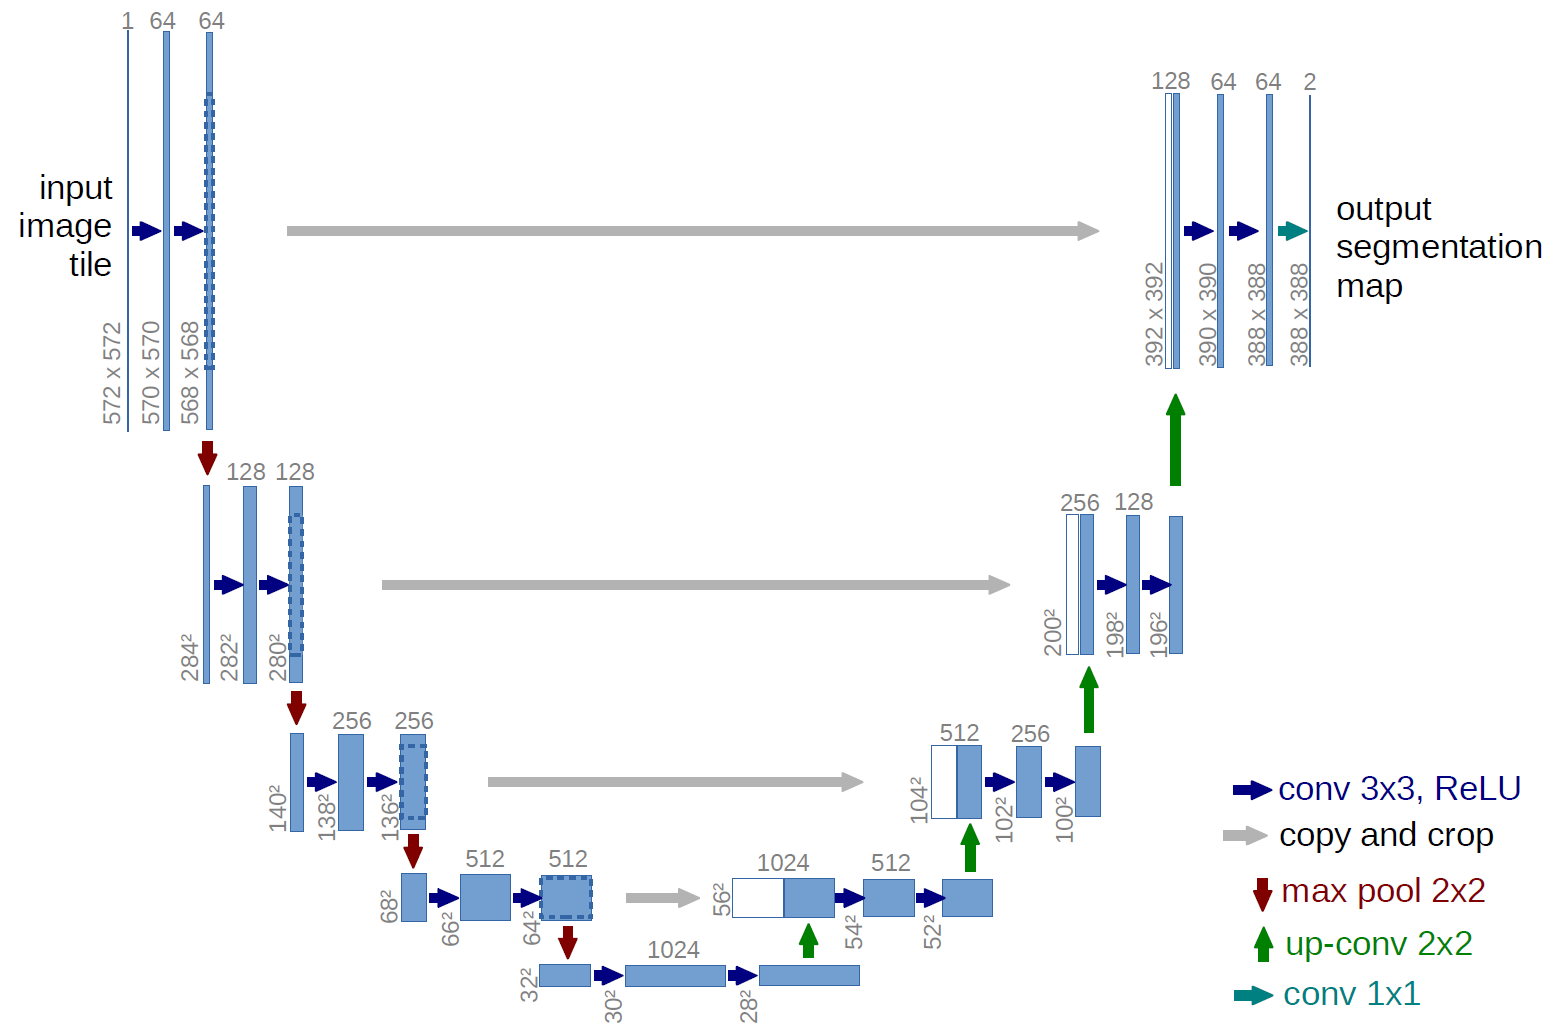
\includegraphics[scale=0.18]{./figs/unetarch.png}
  \caption{U-Net architecture.}
  \label{unetarch}
\end{figure}

\begin{figure}
  \centering
  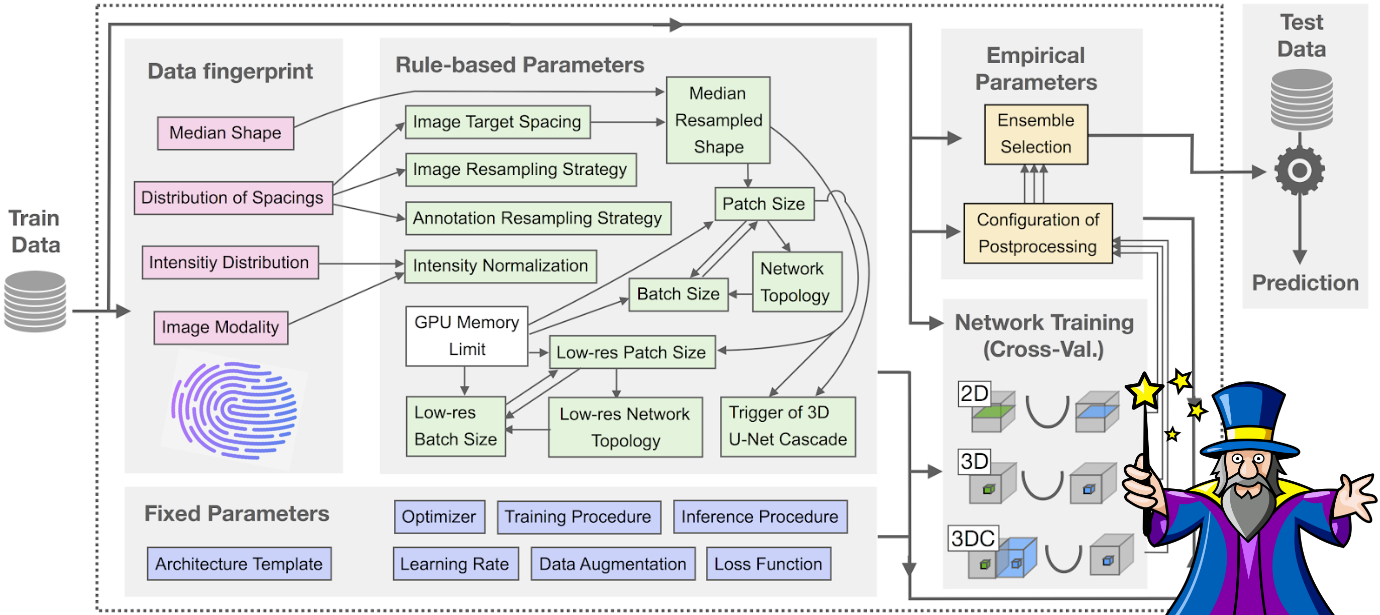
\includegraphics[scale=0.22]{./figs/nnunetarch.png}
  \caption{nnUNet architecture.}
  \label{nnunetarch}
\end{figure}

\section{nnUNet segmentation on hippocampus MRI}

\subsection{Hippocampus}

As shown in Figure \ref{hippoimg} A, a hippocampus comprises Ammon's horn (CA1 --- CA4) and dentate gyrus (2). They are like ropes bundled together to form the hippocampus --- a bundle of ropes. \citet{alves2022imaging} shows that the best modality to image hippocampus is T2-weighted Magnetic Resonance Imaging (MRI), shown in Figure \ref{hippoimg} B. MRI offers good soft tissue contrast deep in brain and is capable to penetrate bones. T2-weighted MRI makes white matter darker than grey matter and shows hippocampus boundary better than T1. Figure \ref{hippoimg} C is T1-weighted MRI in axial view and from it we can see a pair of hippocampus in human brain with head (9), body (10), and tail (11).

There is also CT-based hippocampus imaging, but its low soft tissue contrast requires tracers and more robust CNN model to segment. Ultrasound imaging is an alternative to MRI when it comes to fetal hippocampus, with better spatial resolution at a lower cost.

We obtain the hippocampus MRI data from Medical Segmentation Decathlon held in 2018, as described by \citet{simpson2019large}. The target image covers hippocampus head and body, with three types of labels distinguishing them and background. As shown in Figure \ref{hippolabel}, the head is marked as grey, the body white, and black for background. The main challenge is to segment neighboring hippocampus head and body with high precision.

\begin{figure}
  \centering
  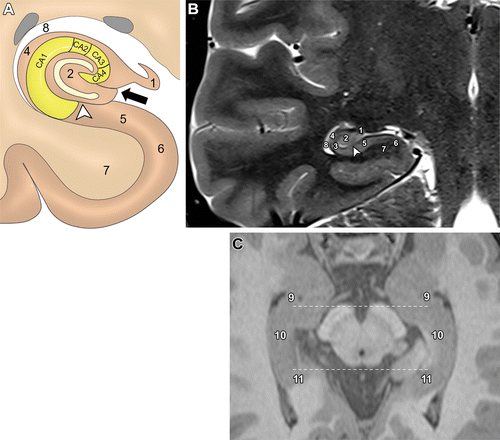
\includegraphics[scale=0.53]{./figs/hippoimg.png}
  \caption{Coronal (A, B) and axial (C) views of hippocampus.}
  \label{hippoimg}
\end{figure}

\begin{figure}
  \centering
  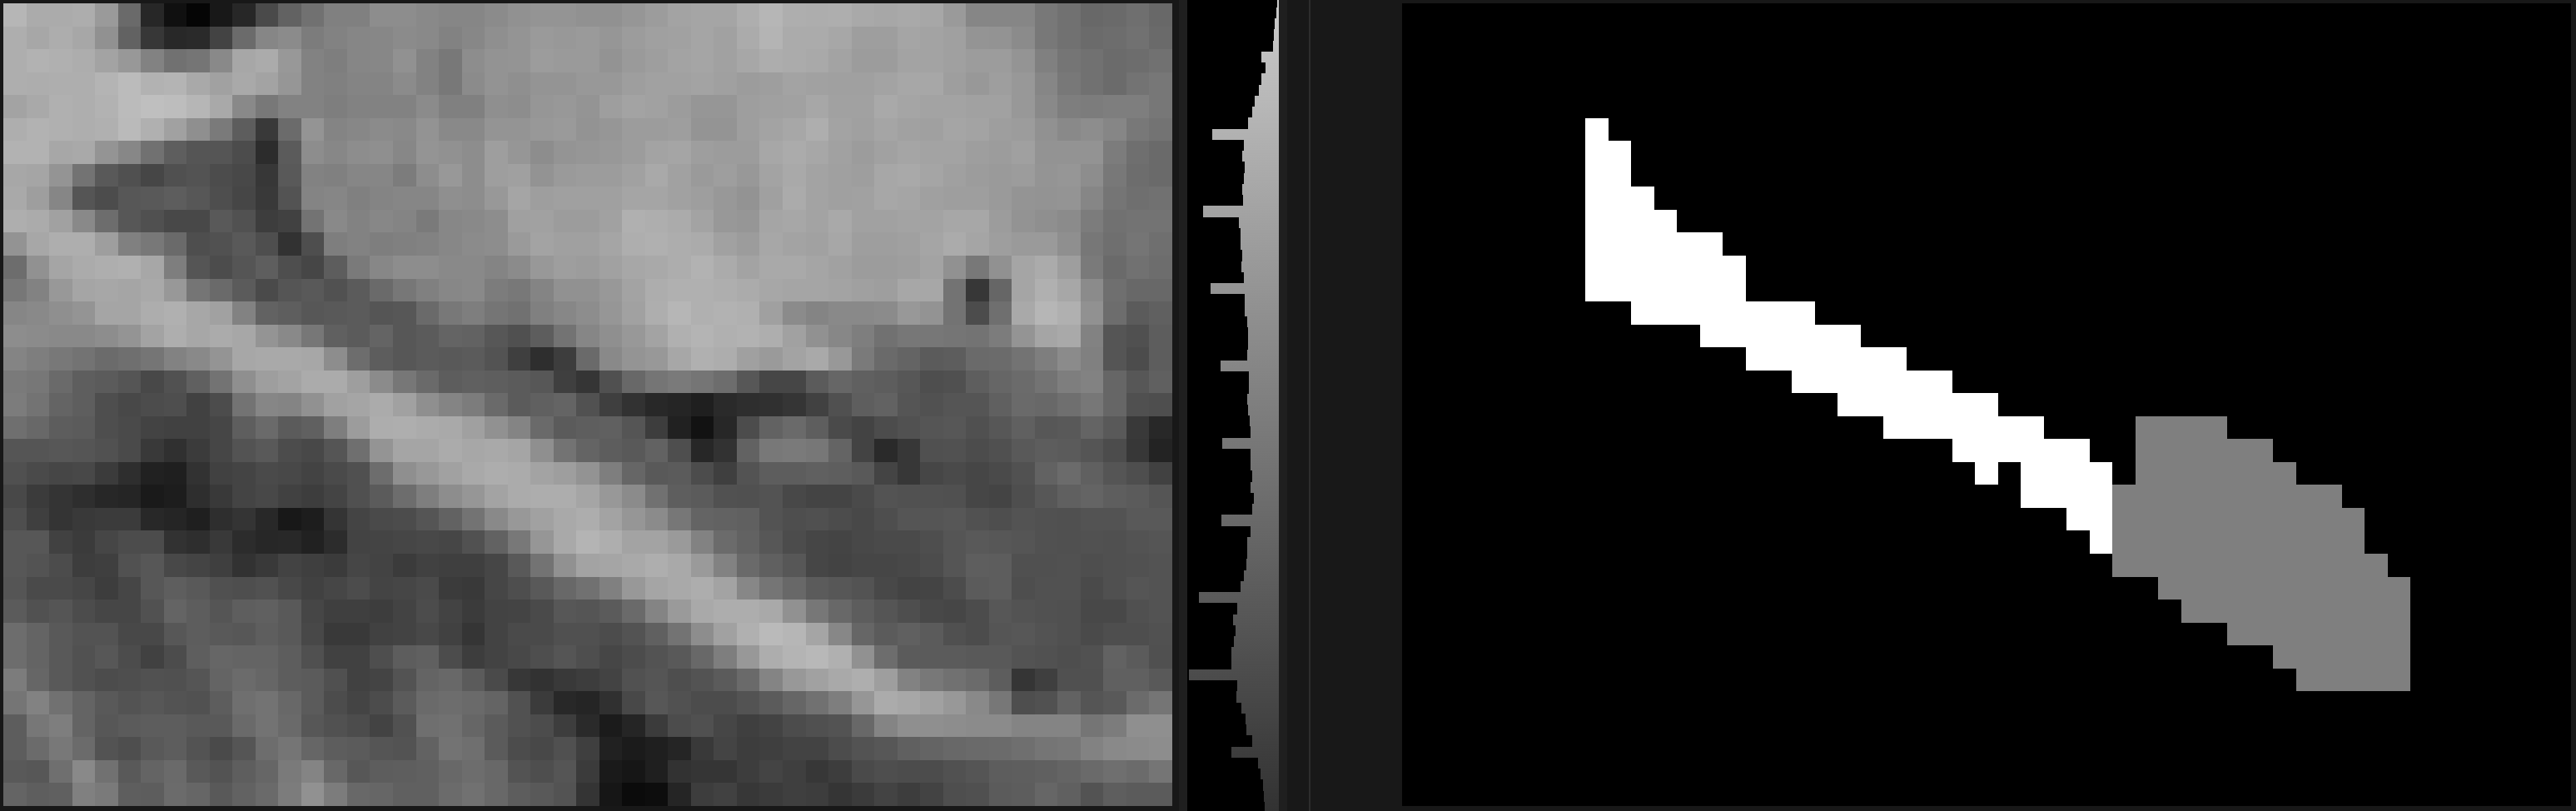
\includegraphics[scale=0.12]{./figs/hippolabel.png}
  \caption{Sagittal view of hippocampus image (left) and label image (right).}
  \label{hippolabel}
\end{figure}

\subsection{Training and testing}

The dataset comprises 260 hippocampus images with 260 label images. We take half of them as test set, and for the other half, we conduct 5-fold cross validation to train our nnUNet model.

\section{Experiment and analysis}

list results as table

\subsection{norm+RELU and RELU+norm and nonorm}



\subsection{early stop of epoches based on sufficient small increment of validation loss}



\section{Discussion and future work}


conclusion, strength and weakness of my contribution, future work to be done on sth.






\begin{table}
  \caption{Sample table title}
  \label{sample-table}
  \centering
  \begin{tabular}{lll}
    \toprule
    \multicolumn{2}{c}{Part}                   \\
    \cmidrule(r){1-2}
    Name     & Description     & Size ($\mu$m) \\
    \midrule
    Dendrite & Input terminal  & $\sim$100     \\
    Axon     & Output terminal & $\sim$10      \\
    Soma     & Cell body       & up to $10^6$  \\
    \bottomrule
  \end{tabular}
\end{table}


\section*{Supplementary Material}

CLI commands

modified codes

\bibliographystyle{abbrvnat}
\bibliography{report}


\end{document}